\chapter{Strategiespiele und Spielregeln}
\label{cha:Strategiespiele und Spielregeln}

In den ersten beiden Unterkapiteln werden die Strategiespiele Tic Tac Toe (Abschnitt \ref{sec:Das Strategiespiel Tic Tac Toe}) und Reversi (Abschnitt \ref{sec:Das Strategiespiel Reversi}) vorgestellt und die Regeln dieser beiden Spiele werden festgelegt. Diese beiden Strategiespiele dienen als Umgebungen für den lernenden Agenten (TD-Q-Agent). Der TD-Q-Agent soll, innerhalb dieser beiden unbekannten Umgebungen, eine möglichst optimale Verhaltensstrategie lernen. \\


\section{Das Strategiespiel Tic Tac Toe}
\label{sec:Das Strategiespiel Tic Tac Toe}

In diesem Abschnitt definieren wir die Regeln des Strategiespiels Tic Tac Toe. Tic Tac Toe ist ein Spiel, welches von genau zwei Spielern gespielt wird. Während eines gesamten Spiels (eine Partie) darf ein Spieler nur Kreuze setzen und der andere Spieler nur Kreise. Wir können uns die Kreuze und Kreise als Spielfiguren vorstellen. Eine Spielfigur die auf das Spielfeld gesetzt wurde, darf seine Position nicht mehr verändern. Das klassische Tic Tac Toe hat 9 Spielfelder (ein 3 x 3 Spielbrett). Innerhalb dieser Arbeit betrachten wir auch ein Tic Tac Toe Spiel mit 16 Spielfeldern (ein 4 x 4 Spielbrett). Der beginnende Spieler muss Kreuzspielfiguren setzen und der nachziehende Spieler Kreisspielfiguren. \\

\paragraph{Spielzüge} jeder Spieler setzt abwechselnd ein Kreuz bzw. einen Kreis in ein Spielfeld des Spielbretts. Eine Spielfigur kann in jedes freie Spielfeld gesetzt werden, außer dieses ist bereits mit einer anderen Spielfigur besetzt. Die Spieler führen solange ihre Spielzüge aus, bis eine Siegesformation eintritt oder alle Spielfelder besetzt sind. 

\paragraph{Ziel des Spiels} ist es, vier Kreuze bzw. vier Kreise in einer bestimmten Position anzuordnen (Siegesformation). Es existieren mehrere unterschiedliche Anordnungsmöglichkeiten von Spielfiguren, die das Spiel beenden und einen Sieg herbeiführen. Bei einem 4 x 4 Spielfeld existieren vier vertikale, vier horizontale und zwei diagonale Anordnungsmöglichkeiten der Spielfiguren, welche einen Sieg herbeiführen würden. Insgesamt zehn verschiedene Siegesanordnungen für beide Spieler. Sind alle Spielfelder besetzt und für keinen der Spieler ist eine Siegesformation aufgetreten, dann gewinnt beziehungsweise verliert keiner der beiden Spieler und es entsteht ein Unentschieden. \\

\begin{figure}[!htbp]
  \centering
  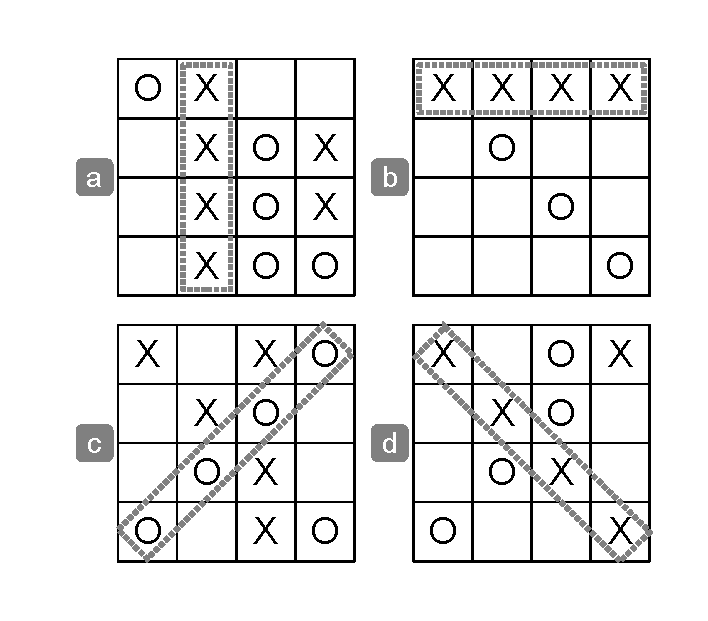
\includegraphics[scale = 0.6]{inhalt/abbildungen/siegesbedingungen_tictactoe.pdf}
  \caption{Tic Tac Toe Siegesformationen für den Kreuzspieler.}
  \label{fig:siegesbedingungen_tictactoe}
\end{figure}

Vier mögliche Siegesformationen sind in Abbildung \ref{fig:siegesbedingungen_tictactoe} dargestellt. (a) Kreuz gewinnt, mit einer vertikalen Siegesformation. (b) Kreuz gewinnt, mit einer horizontalen Siegesformation. (c) Kreuz gewinnt, mit einer diagonalen Siegesformationen. (d) Kreuz gewinnt, mit einer diagonalen Siegesformation.

\section{Das Strategiespiel Reversi}
\label{sec:Das Strategiespiel Reversi}
In diesem Abschnitt definieren wir die Regeln des Strategiespiels Reversi. Reversi ist ein komplexeres Strategiespiel als Tic Tac Toe, weil Reversi 64 Spielfelder (ein 8 x 8 Spielbrett) hat. Das Reversi Spielbrett ist um den Faktor 4 größer, als das 4 x 4 Tic Tac Toe Spielbrett. \\

Reversi oder auch Othello genant, ist ein Spiel für zwei Personen die gegeneinander antreten. Eine Person setzt weiße runde Spielsteine und die andere Person schwarze runde Spielsteine. Jede neue Partie Reversie beginnt im selben Ausgangszustand (siehe Abbildung \ref{fig:ausgangssituation_reversi}). Die Spieler setzen nacheinander genau einen Spielstein und einmal gesetzte Spielsteine können ihre Position nicht mehr verändern. \\

Anmerkung zu Abbildung \ref{fig:ausgangssituation_reversi}  Die äußeren weiß hinterlegten Reihen, in denen sich Zahlen befinden, dienen dazu, die Positionen der einzelnen Spielfelder genau zu definieren. In der Ausgangsspielsituation befinden sich bereits 2 weiße Spielsteine, an den Positionen (3,4) und (4,3) und zwei schwarze Spielsteine, an den Positionen (3,3) und (4,4). \\

\begin{figure}[!htbp]
  \centering
  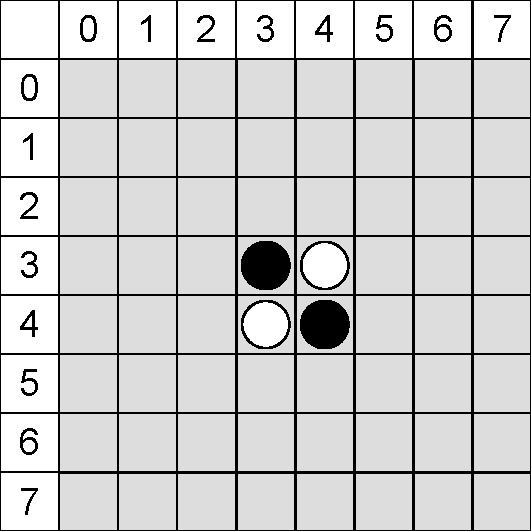
\includegraphics[scale=0.5]{inhalt/abbildungen/ausgangssituation_reversi.pdf}
  \caption{Ausgangsspielzustand Reversi.}
  \label{fig:ausgangssituation_reversi}
\end{figure}

Eine Spielregel von Reversi ist, dass gesetzte Spielsteine ihre Farbe ändern können, wenn sie vertikal, horizontal oder diagonal von einem Spielstein des Gegenspielers eingeschlossen werden. Dann wechseln die Spielsteine ihre Farbe und gehören dem Gegenspieler. Ein korrekter Spielzug muss immer mindestens einen gegnerischen Spielstein erobern. 

Weiterhin  darf ein Spielstein nur dann gesetzt werden, wenn ein anderer Spielstein, in einer diagonalen, vertikalen oder horizontalen Linie, existiert. Es dürfen auch keine freien Felder zwischen dem zu setzenden Steinen liegen. \\

\begin{figure}[!htbp]
  \centering
  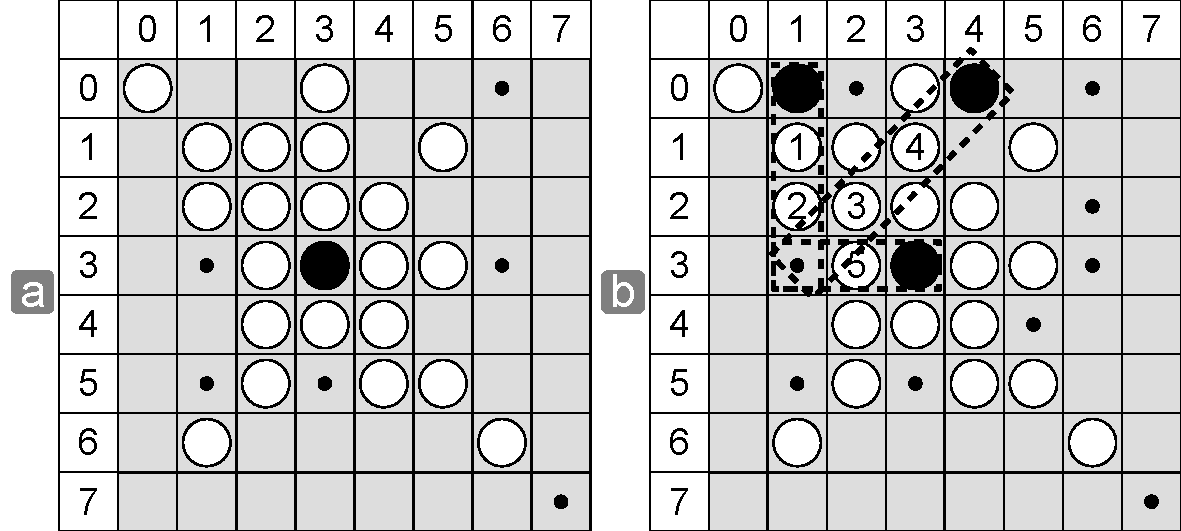
\includegraphics[scale=0.5]{inhalt/abbildungen/zuege_schwarz_reversi.pdf}
  \caption{Fortgeschrittene Spielzugmöglichkeiten Reversi.}
  \label{fig:zuege_schwarz_reversi}
\end{figure}

Anmerkung zu Abbildung \ref{fig:zuege_schwarz_reversi}, diese zeigt zwei möglicherweise auftretende Spielsituationen, die einzig verdeutlichen sollen, welche Zugmöglichkeiten der Spieler mit den schwarzen Spielsteinen hat und warum nur diese Züge möglich sind. Die kleinen schwarzen Punkte zeigen die Positionen an denen ein schwarzer Spielstein gesetzt werden darf. (a) Eine fortgeschrittene Spielsituation mit maximal einem möglichen schwarzen Spieltein. (b) Eine Spielsituation mit maximal 3 möglichen schwarzen Spielsteinen für die Position (3,1). \\

Abbildung \ref{fig:zuege_schwarz_reversi} zeigt zwei verschiedene Reversi Spielsituationen (Schwarz ist am Zug). Die kleinen schwarzen Punkte symbolisieren zulässige Spielzüge. In Spielsituation (a) hat Spieler Schwarz genau 6 Spielzugmöglichkeiten. In jedem dieser Spielzüge erobert er mindestens einen weißen Spielstein und die Reihe wird nicht durch einen schwarzen Spielsein unterbrochen. In Spielsituation (b) hat Spieler Schwarz 9 Spielzugmöglichkeiten. Das setzen eines Spielsteins auf Position (3, 1) würde dem schwarzen Spieler 5 weiße Spielsteine einbringen, da mehrere schwarze Spielsteine diagonal, horizontal und vertikal an diese Position angrenzen. Die 5 eroberten weißen Spielsteine würden dann die schwarze Spielfarbe annehmen. \\

\paragraph{Ziel des Spiels} ist es, am Ende des Spiels mehr Spielsteine seiner eigenen Farbe zu haben, als der Gegner Spielsteine in seiner Farbe hat. Das Spiel endet, wenn keiner der beiden Spieler mehr einen Spielstein, nach den Regeln des Spiels, auf das Spielbrett setzen kann. \\